\documentclass{article}[12pt]

\usepackage[utf8]{inputenc}
\usepackage{graphicx}
\usepackage{subcaption}
\usepackage{float}
\usepackage[a4paper, margin=1in]{geometry}
\usepackage{hyperref}

\graphicspath{./images/}

\title{Création d’une plateforme pour l’analyse du signal posturographique \\
\textbf{premier jet}}
\author{Inès PINGAULT, Anaëlle MAZOUNI, Hippolyte DEPARIS \\
Lille }
% \texttt{andyr@comp.leeds.ac.uk}
\date{\today}

\begin{document}
\maketitle

\newpage
\tableofcontents

\newpage
\section{Introduction}

La posturographie, aussi appelée posturologie, est une technique employée pour évaluer, 
mesurer et contrôler la posture en position debout. Pour maintenir un équilibre vertical, 
le corps humain ajuste en permanence sa posture par rapport à son environnement en fonction de 
certains signaux qu'il reçoit. Ces signaux sont captés par les yeux, la colonne vertébrale, 
l’oreille interne ou encore les pieds. Le cerveau les analyse et envoie des instructions au 
corps dans le but de modifier sa posture en temps réel aux différents éléments perçus. Si ces 
signaux, importants pour le maintien de l'équilibre ne sont pas ou mal perçus, ou mal analysés,
la posture ne sera pas correctement adaptée, et des troubles tels que des déséquilibres, des 
vertiges ou encore des problèmes musculosquelettiques pouvant aller jusqu'à des douleurs 
chroniques dans certaines régions de l’organisme pourraient apparaître. Il est donc important 
pour les posturologues de mettre aujourd’hui l’accent sur l'étude du rôle des yeux, des pieds 
ainsi que les occlusions dentaires dans les problèmes liés à la posture. Cette discipline étudie
la position de l’homme dans l’espace (son équilibre, sa stature, son aplomb, sa stabilité...)
grâce à des appareils de mesure spécialisés. Elle prend en compte la capacité de rester en 
équilibre sur ses pieds ainsi que la symétrie du corps ou la perception visuelle de 
l'horizontalité. Ces études sont possibles aussi bien dans des situations statiques que 
dynamiques. La posturographie dynamique informatisée (non étudiée dans ce rapport) est une 
technique d’évaluation clinique non invasive permettant de quantifier les mécanismes
d’adaptation du système nerveux central lorsque le corps est en mouvement (Figure 1).  
La posturographie statique évalue quant à elle la posture d’un patient en équilibre
orthostatique (position érigée immobile, fondamentale de l'espèce humaine). Cette évaluation
se fait en positionnant debout, le patient sur une plateforme équipée de nombreux capteurs 
de pression. L’enregistrement des oscillations du centre de pression des pieds permettent 
de retracer l'évolution du centre de gravité (ou centre de masse) du patient. Lors de ces 
évaluations, on étudie aussi la réponse posturale du patient à certaines perturbations 
(Figure 2).


\begin{figure}[ht]
    \centering
    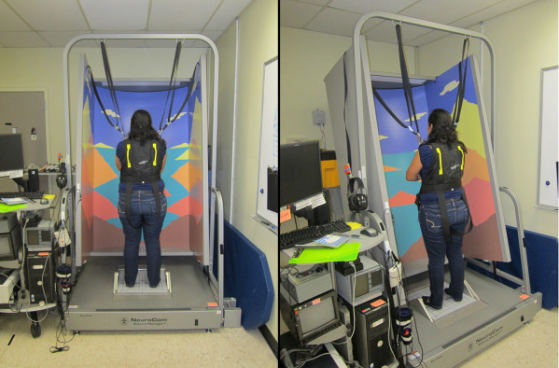
\includegraphics[width=0.5\textwidth]{images/introduction/dynamique.png}
    \caption{Machine d’analyse de la posturographie dynamique }
    \label{fig:posturographie-dynamique}
\end{figure}

\begin{figure}[ht]
    \centering
    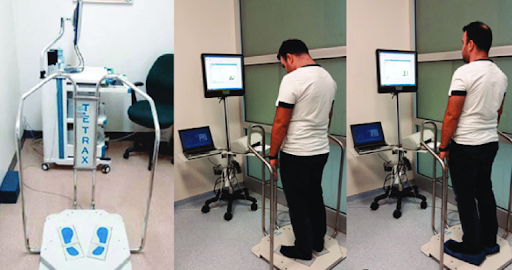
\includegraphics[width=0.5\textwidth]{images/introduction/statique.png}
    \caption{Machine d’analyse de la posturographie statique }
    \label{fig:posturographie-statique}
\end{figure}



\newpage
\section{Différents types de signaux}

Il existe plusieurs types de signaux étudiés en posturographie, à l'aide de différents instruments.

\subsection{Les forces et moments}

Les forces sont les interactions mécaniques exercées par les pieds du patient sur la \textbf{surface d'une plateforme de mesure}.
Ces forces sont mesurées dans les trois directions de l'espace : 
\begin{itemize}
  \item $F_x$ : force horizontale le long de l'axe $x$
  \item $F_y$ : force horizontale le long de l'axe $y$ 
  \item $F_z$ : force verticale, perpendiculaire à la surface (poids corporel ou force de gravité)
\end{itemize}
Ici, les forces $F_x$ et $F_y$ caractérisent les efforts de contrôle postural pour maintenir l'équilibre 
en gérant les déplacement latéraux ($x$) et avant-arrière ($y$).
$F_z$ caractérise la force exercée par le poids du corps sur la plateforme. Elle varie 
lors des mouvements dynamiques (e.g. sauts, marches ou transitions).

Les moments sont les forces de rotations générées autour des axes principaux de la plateforme.
Ils mesurent les rotations produites par les forces appliquées par le corps.
Les moments sont aussi mesurés dans les trois directions de l'espace : 

\begin{itemize}
  \item $M_x$ : moment autour de l'axe $x$, reflétant les rotations dans le plan frontal (inclinaison latérale du corps)
  \item $M_y$ : moment autour de l'axe $y$, indiquant les rotations dans le plan sagittal (basculement avant-arrière du corps)
  \item $M_z$ : moment autour de l'axe $z$, mesurant les rotations 
\end{itemize}

Les moments donnent des informations sur les ajustements posturaux, comme un déséquilibre latéral ($M_x$) 
ou une bascule avant-arrière ($M_y$) peut indiquer des stratégies de compensation. La torsion du corps ($M_z$) en réponse à un mouvement ou à une perturbation.

Les résultantes égales et opposées des forces agissant sur la masse corporelle s'appliquent respectivement au centre de gravité et au centre de pression.

L'équilibre est atteint à la condition que ces deux points soient alignés sur la même verticale.

\begin{figure}[h]
  \centering
  \begin{subfigure}[b]{0.45\textwidth}
    \centering
    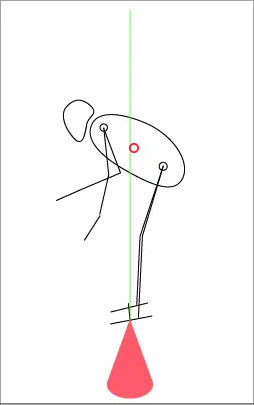
\includegraphics[height=5cm]{images/tactique-cdg.png}
    \caption{Tactique CDG}
    \label{fig:tactique_cdg}
  \end{subfigure}
  \hfill
  \begin{subfigure}[b]{0.45\textwidth}
    \centering
    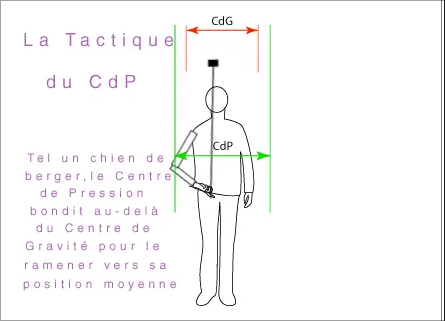
\includegraphics[height=5cm]{images/tactique-cdp.png}
    \caption{Tactique CDP}
    \label{fig:tactique_cdp}
  \end{subfigure}
  \caption{Différentes tactiques}
  \label{fig:2_tactiques}
\end{figure}

Ces mesures servent à l'analyse des oscillations posturales (statiques et dynamiques) et permettent d'évaluer la répartition du poids entre les deux pieds.

\subsection{Accélération et vitesses angulaires (Centrales inertielles, IMU)}

Les \textbf{accélérations} mesurent les variations de vitesse des segments corporels dans les trois axes de l'espace ($x$,$y$,$z$). 
Ces mesures sont réalisées par des \textbf{accéléromètres}, qui détectent les forces d'accélération appliquées au corps ou à ses \textit{segments}. 
Cela permet d'identifier les changements rapides dans dynamique corporelle, comme lors d'un déséquilibre ou d'une activité physique intense.

Les \textbf{vitesses angulaires} mesurent les rotations des segments corporels autour des axes principaux (pitch, roll, yaw). 
Capturées par des gyroscopes, ces données renseignent sur l’amplitude et la vitesse des mouvements rotatifs (par exemple, une rotation du tronc ou de la tête).
On s'en sert pour analyser les stratégies d'ajustement postural ou les mouvements complexes.

Avec ces deux types de signaux, on peut en déduire la \textit{stabilité dynamique}, qui permet de comprendre les micro-enregistrements permettant le maintien de l'équilibre dans des environnements dynamiques, et la mesure de la qualité des réponses posturales à des perturbations externes.
Ces signaux permettent également de suivre précisément les déplacements et rotations des segments corporels (les membres, le tronc, la tête...) afin d'évaluer les asymétries ou déséquilibres.

Ces mesures sont utilisées dans diverses situations.
Elles sont utilisées pour mesurer les progrès dans la récupération posturale ou locomotrice (e.g. après une blessure, un AVC).
Elles permettent également d'analyser les performances athlétiques des mouvements dans des environnements non contrôlés,
comme les terrains de sport ou les espaces naturel athlétiques des mouvements dans des environnements non contrôlés, comme les terrains de sport ou les espaces naturels.

Des machines spécialisées existent pour suivre et mesurer ces signaux:
\begin{itemize}
  \item \textbf{Xsens MTw Awinda} : capture les accélérations et vitesses angulaires pour \\ une analyse cinématique complète.
  \item \textbf{Noraxon MyoMotion} : fournit des mesures détaillées des mouvements segmentaires en \\ intégrant des capteurs inertiels.
  \item \textbf{IMU portables (Shimmer, Delsys)} : capteurs légers fixés sur le tronc, les membres ou la tête pour des analyses mobiles.
\end{itemize}

\begin{figure}[ht]
  \begin{center}
    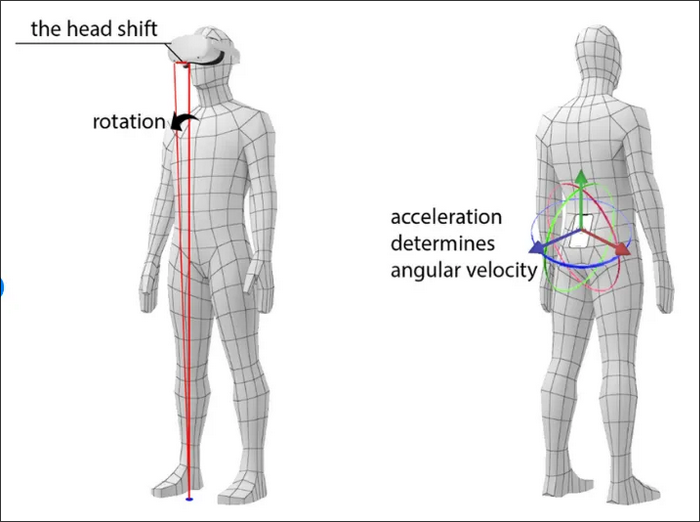
\includegraphics[width=0.5\textwidth]{images/legende.png}
  \end{center}
  \caption{Légende à trouver}\label{fig:legende}
\end{figure}

\subsection{Pressions plantaires (Systèmes de baropodométrie)}

Les \textbf{pressions plantaires} mesurent la répartition des forces sous les pieds au niveau des zones d'appui. 
Ces pressions sont capturées par des capteurs disposés sur une surface ou intégrés dans des semelles.
Ces mesures permettent d'identifier les points de pression maximale et minimale, fournissant des données sur la statique et la dynamique du pied.

Les \textbf{centres de pression} sont calculés à partir des variations de pression. Ils reflètent les ajustements dynamiques de la posture en réponse aux déséquilibres.

Les mesures de ces signaux nous permettent de \textbf{cartographier} les zones d'appui de visualiser les charges appliquées sur les pieds. 
On peut alors identifier les zones à risque de pathologie (comme l'hallux valgus ou la fasciite plantaire).
On peut également analyser la dynamique du pied, c'est-à-dire analyser les phases d'appui et de propulsion pendant la marche ou la course.
L'évaluation des déséquilibres ou anomalies dans la distribution des forces est alors possible.

Ces études sont appliquées en podologie et orthopédie, pour détecter les troubles plantaires ou les anomalies posturales.
Elles sont aussi utilisées pour suivre les progrès post-blessures ou post-chirurgie de patients.
Enfin, on peut aussi les mener dans le but d'optimiser les performances athlétiques en analysant les impacts au sol.

Ces mesures sont rendues possibles grâce à des machines spécialisées : 
\begin{itemize}
  \item \textbf{Tekscan F-scan} : plateforme baropodométrique pour analyse en statique et dynamique
  \item \textbf{Zebris FDM} : Système baropodométrique avancé utilisé en rééducation et recherche.
  \item \textbf{Semelles capturant les pressions (Moticon)} : Capteurs intégrés pour une analyse mobile.
\end{itemize}

\begin{figure}[H]
  \centering
  \begin{subfigure}[b]{0.4\linewidth}
    \centering
    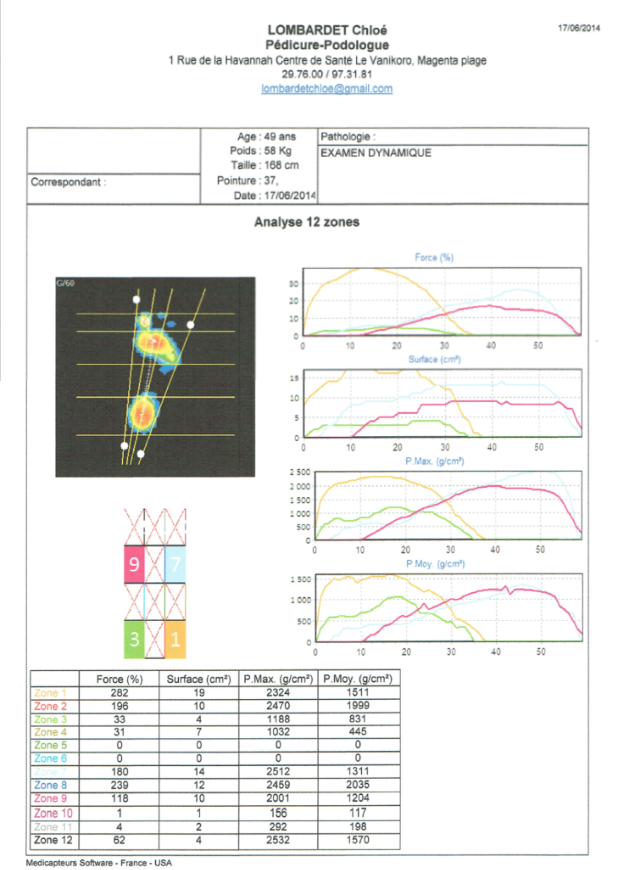
\includegraphics[width=\textwidth, height=10cm]{images/analyse_12_zone.png}
    \caption{Analyse en 12 zones}
    \label{fig:analyse_12_zone}
  \end{subfigure}
  \hspace{0.03\textwidth}
  \begin{subfigure}[b]{0.4\linewidth}
    \centering
    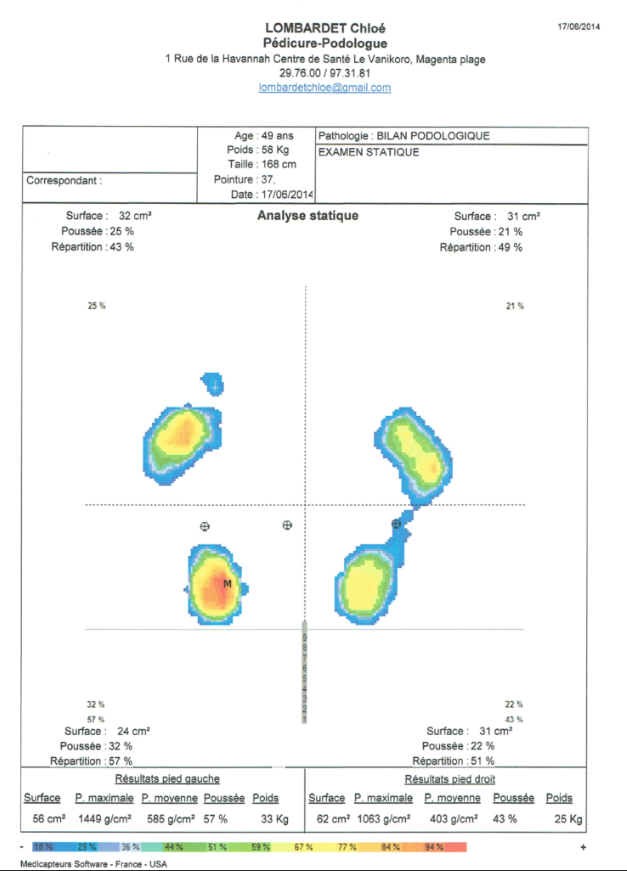
\includegraphics[width=\textwidth, height=10cm]{images/analyse_statique.png}
    \caption{Analyse statique}
    \label{fig:analyse_statique}
  \end{subfigure}
  \begin{subfigure}[b]{0.4\linewidth}
    \centering
    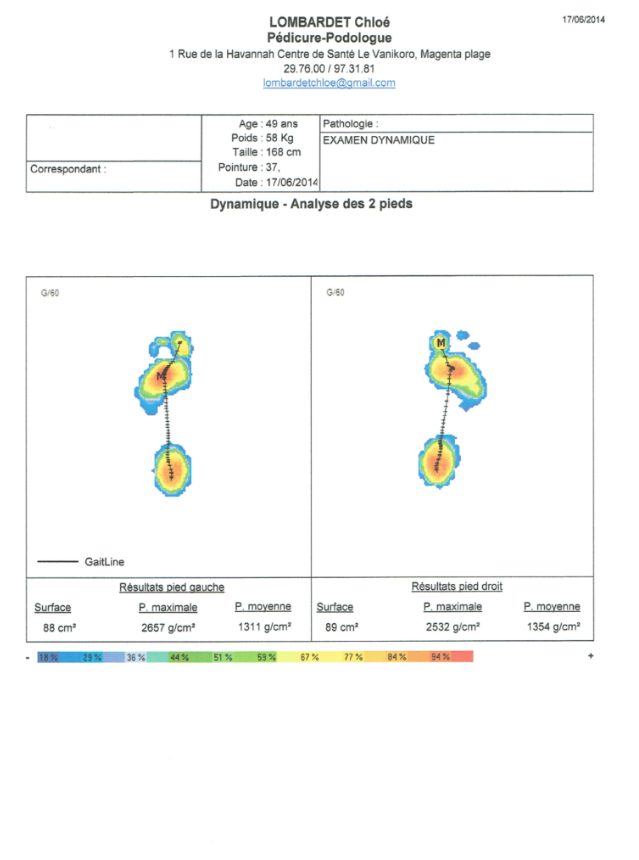
\includegraphics[width=\textwidth, height=10cm]{images/analyse_2_pieds.png}
    \caption{Analyse des deux pieds}
    \label{fig:analyse_2_pieds}
  \end{subfigure}
  \caption{Rapports de différents types d'analyse}
  \label{fig:3_type_analyse}
\end{figure}

\subsection{Potentiels électriques musculaires (EMG - Électromyographie)}

Les \textbf{potentiels électriques musculaires} sont utilisés pour mesurer l'activité électrique
générée par les muscles lors de leurs contractions. Ces signaux sont enregistrés avec des électrodes de surface ou intramusculaires.
Les signaux EMG reflètent l'intensité et la durée d'activation musculaire.
Ces signaux sont influencés par le recrutement des fibres musculaires et leur fréquence de décharge.
Les données EMG permettent de suivre l'ordre d'activation des muscles et leur coordination.

L'étude de ces données nous permet de mesurer l'effort des groupes musculaires en réponse à des tâches posturales ou locomotrices.
Elle nous permet également de mieux identifier les synergies musculaires et les déséquilibres entre muscles agonistes et antagonistes.

Ces analyses sont notamment réalisées dans le cadre de détection des troubles neuromusculaires (par exemple, faiblesse musculaire ou spasticité).
Elles sont aussi performées dans le but d'analyser des stratégies musculaires afin d'optimiser les performances.
Finalement, ces données sont aussi récoltées pour le suivi de la récupération musculaire après des blessures ou des interventions chirurgicales.
 
Ces mesures sont rendues possibles grâce à des machines spécialisées : 
\begin{itemize}
  \item \textbf{Delsys Trigno} : fournit des enregistrements sans fil haute résolution de l’activité musculaire.
  \item \textbf{Noraxon Ultium EMG} : Utilisé pour une analyse avancée en sport et en biomécanique.
  \item \textbf{BTS FREEEMG} : Un système sans fil permettant une analyse complète de l’activation musculaire.
\end{itemize}

\begin{figure}[ht]
  \centering
  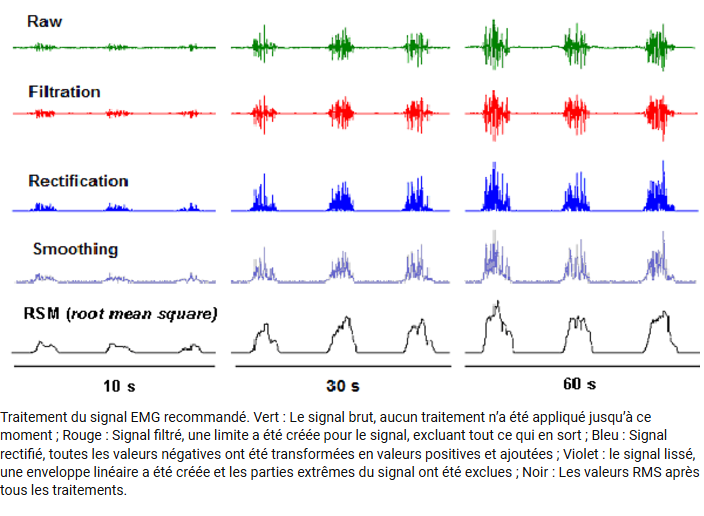
\includegraphics[width=0.5\textwidth]{images/emg.png}
  \caption{Exemple de signal EMG relevé}\label{fig:emg}
\end{figure}


\subsection{Trajectoires segmentaires (systèmes de capture vidéo 3D)}

Les \textbf{trajectoires tridimensionnelles} sont des signaux utilisés pour mesurer les déplacement des segments corporels (membres, tronc, tête) dans les trois axes de l'espace.
Il sont capturés à l'aide de caméras et de marqueurs placés sur le corps.

Les \textbf{angles articulaires} sont calculés à partir de trajectoires segmentaires pour évaluer les amplitudes de mouvement.

À l'aide de ces deux signaux, on peut recréer une cinématique détaillée, qui est un suivi précis des mouvements segmentaires et des angles articulaires.
Ils permettent aussi d'évaluer les asymétries ou anomalies de mouvements, utiles dans le diagnostic des troubles musculo-squelettiques.

L'analyse de ces signaux est effectuée en recherche clinique, dans l'étude de la cinématique du mouvement d'un patient atteint de troubles neurologiques ou orthopédique.
Elle est également faite à des fins d'optimisation des mouvements d'un athlète, afin d'améliorer sa performance.
Elle est aussi utilisée pour suivre les progrès post-blessure ou post-chirurgie d'un patient en réhabilitation.

Ces analyses sont rendues possible grâce à ces machines spécialisées : 
\begin{itemize}
  \item \textbf{Vicon} : système de capture de mouvements de haute précision pour une analyse en 3D.
  \item \textbf{OptiTrack} : fournit des solutions flexibles pour la cinématique du mouvement.
  \item \textbf{Qualisys} : système avancé pour capturer et analyser les mouvements complexes.
\end{itemize}

\begin{figure}[ht]
  \begin{center}
    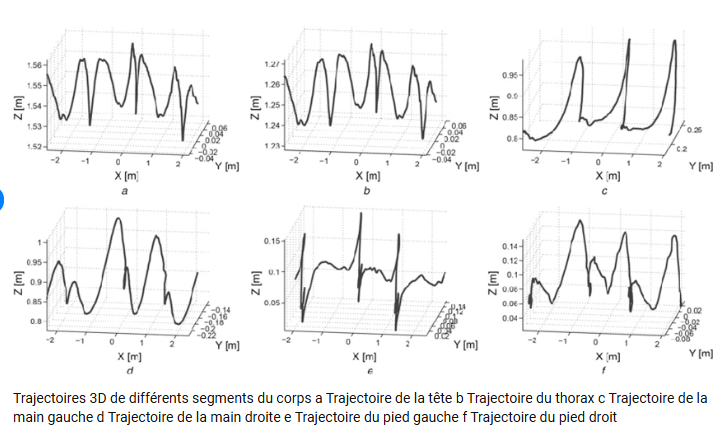
\includegraphics[width=0.5\textwidth]{images/trajectoires_3D.png}
  \end{center}
  \caption{Trajectoires tridimensionnelles de différents segments du corps}\label{fig:trajectoires_tridimensionnelles}
\end{figure}

\subsection{Paramètres spatio-temporels (pistes de marche électronique)}

On cherche à mesurer la \textbf{vitesse moyenne} de la marche ou de la course, ainsi que la \textbf{longueur du pas}, c'est-à-dire la distance parcourue entre deux appuis successifs d'un même pied.
On mesure également la \textbf{cadence} (en unité de temps), et le \textbf{temps de contact au sol}.

Ces données nous permettent d'analyser la marche, ce qui est utilisé pour évaluer la régularité et l'efficacité du mouvement.
Ces données nous assistent aussi dans l'identification des anomalies de la marche liées à des conditions neurologiques, musculo-squelettiques ou orthopédique.o

Ces signaux sont exploités en clinique dans le diagnostic des troubles de la démarche (e.g. après un AVC, ou en cas de maladie de Parkinson).
Elles se révèlent utiles dans le suivi des progrès des patients en rééducation.
Également, l'analyse de la foulée est pratiqué dans le domaine sportif afin d'améliorer les performances des coureurs.

L'analyse de ces signaux est rendue possible par ces machines spécialisées :
\begin{itemize}
  \item \textbf{GAITRite} : fournit des mesures spatio-temporelles précises via des tapis électroniques.
  \item \textbf{Zebris FDM-T} : Intègre la baropodométrie pour une analyse complète de la marche.
  \item \textbf{MotionMetrix}: Capture les paramètres spatio-temporels et les intègre dans une analyse globale du mouvement
\end{itemize}


\begin{figure}[ht]
  \centering
  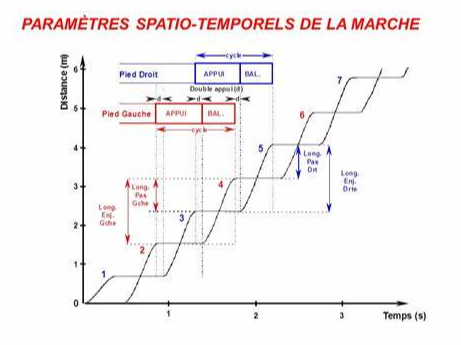
\includegraphics[width=0.5\textwidth]{images/activites_posturo_cinetiques.png}
  \caption{Paramètres spatio-temporels de la marche}\label{fig:parametres_spatio_temporels}
  \label{fig:spatio_temporels_marche}
\end{figure}

\begin{figure}[ht]
  \centering
  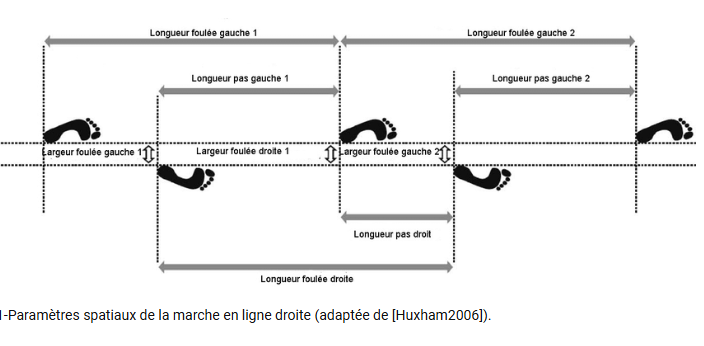
\includegraphics[width=0.5\textwidth]{images/spatio-temporels-ligne-droite.png}
  \caption{Paramètres spatiaux de la marche en ligne droite}
  \label{fig:param_spatiaux_ligne_droite}
\end{figure}


\newpage
\section{Enregistrement des signaux}

\subsection{Enregistrement des forces et moments sur une plateformes de force}

Les plateformes de force sont équipées des “capteurs de force”. 
Des jauges de contrainte ou des capteurs piézoélectriques sont intégrés dans leur structure.
Ces capteurs permettent de mesurer les composantes des forces et des moments exercés sur la plateforme.
Les données capturées sont transmises à un système d’acquisition numérique (DAQ, pour Data Acquisition System), par connexion filaires ou sans fil.
Ce système convertit les signaux analogiques en données numériques prêtes à être exploitées.

Ces plateformes sont en général couplées à des logiciels comme \textit{NetForce} pour AMTI ou \textit{BalanceTest} pour Bertec. 
Ces logiciels calculent des indicateur spécifiques tel que le Centre de Pression (CdP) permettant alors de visualiser les données en temps réel.

\subsection{Enregistrement des accélérations et vitesses angulaires (IMU)}

Les IMU contiennent des accéléromètres pour les accélérations linéaires, des gyroscopes pour mesurer les rotations angulaires, et certaines fois des magnétomètres pour obtenir l’orientation absolue.
Les capteurs utilisés sont fixés via des bandes d’élastiques ou des adhésifs sur de segments corporels clés comme le tronc, les membres supérieurs et inférieurs.
La transmission des données vers l’ordinateur ou l’enregistreur portable se fait via Bluetooth ou Wi-Fi permettant alors une acquisition en temps réel des données.

Les données brutes sont ensuite traitées avec les logiciels comme \textit{MVN Analyze} pour Xsens et \textit{Noraxon MR3} qui vont traiter les données brutes pour fournir des informations comme les trajectoires, les vitesses angulaires, et les accélérations.

\subsection{Enregistrement des pressions plantaires (Systèmes de baropodométrie)}

Les systèmes de baropodométrie utilisent des capteurs capacitifs ou résistifs intégrés dans des plateformes ou dans des semelles.
Ces capteurs vont permettre de mesurer les variations de pression sur la surface plantaire. On récupère les signaux via des connecteurs câblés ou des dispositifs sans fil directement intégrés dans la plateforme ou dans les semelles. 

Pour traiter ses données on va souvent utiliser les logiciels comme \textit{Tekscan Research Software} ou \textit{Zebris FDM}.
Les résultats seront souvent sous forme de carte de pression plantaires et des trajectoires du CdP.

\subsection{Enregistrement des potentiels électriques musculaires (EMG)}

On va placer des électrodes directement sur la peau au-dessus des muscles ciblésn ou on l’insère dans les muscles pour des mesures précises.
Les signaux électriques capturés sont de faible amplitude et nécessitent un passage via un amplificateur EMG.
On va pouvoir utiliser les logiciels dédiés comme \textit{EMGworks}, \textit{Noraxon MR3} qui filtrent et analysent les données pour en extraire les caractéristiques musculaires comme l’intensité, la durée, la fréquence.

\subsection{Enregistrement des trajectoires segmentaires (Systèmes vidéo 3D)}

On va placer des marqueurs réfléchissants avec des LEDs qui sont placés sur des points anatomiques spécifiques comme les articulations et les segments corporels.
Les caméras infrarouges ou optiques suivent les marqueurs en mouvement. 
Les données sont collectées en temps réel par un logiciel comme Nexus pour Vicon ou Motive pour OptiTrack.
Ils reconstruisent les trajectoires 3D des segments corporels et calculent les angles articulaires.


\subsection{Enregistrement des paramètres spatio-temporels (Systèmes filaires et tapis électroniques)}

Les tapis électroniques sont équipés de capteurs qui détectent la pression ou l’impact de chaque pas.
Ils mesurent différents paramètres comme la cadence, la vitesse de marche, la longueur de pas, et la symétrie des appuis.
On va, là aussi, utiliser les logiciels comme \textit{GAITRite} ou \textit{Zebris FDM-T} qui génèrent des rapports complets sur la dynamique de la marche.


\newpage
\section{Les différentes machines}

\subsection{Plateformes de force}

Ces plateformes mesurent les forces appliquées par les pieds sur leur surface grâce à des capteurs, basés sur des jauges de contrainte ou des capteurs piézoélectriques. 
Ces capteurs enregistrent les composantes des forces dans les trois axes (X, Y, Z) et les moments de force autour de ces axes. 
Les données relevées permettent de calculer le \textbf{Centre de Pression (CdP)}, reflétant la répartition du poids et des ajustements posturaux du corps. 
Le CdP est alors suivi en temps réel dans le but d'analyser les oscillations posturales.

Elles sont fréquemment utilisées pour évaluer l’équilibre postural, la répartition du poids ainsi que les ajustements dynamiques du corps. 
Elles sont essentielles dans des domaines comme la neurologie (troubles de l’équilibre), la rééducation (suivi de récupération post-blessure), et le sport (analyse de la performance ou de l’impact). 
Ces dispositifs contribuent également à identifier les asymétries et à évaluer le risque de chute chez les personnes âgées.

\subsubsection{Exemples (liens) :}
\begin{itemize}
  \item \href{https://www.amti.biz/product-line/force-plates/}{\textbf{AMTI AccuSway Plus}}
  \item \href{https://www.bertec.com/products/force-plates}{\textbf{Bertec Force Plate}}
\end{itemize}

\begin{figure}[ht]
  \centering
  \begin{subfigure}[b]{0.45\textwidth}
    \centering
    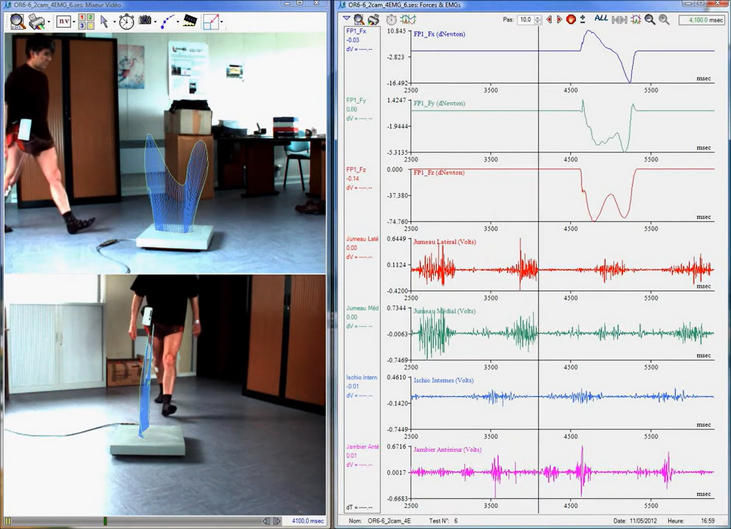
\includegraphics[height=5cm]{images/OR6.png}
    \caption{Logiciel OR6}\label{fig:OR6}
  \end{subfigure}
  \begin{subfigure}[b]{0.45\textwidth}
    \centering
    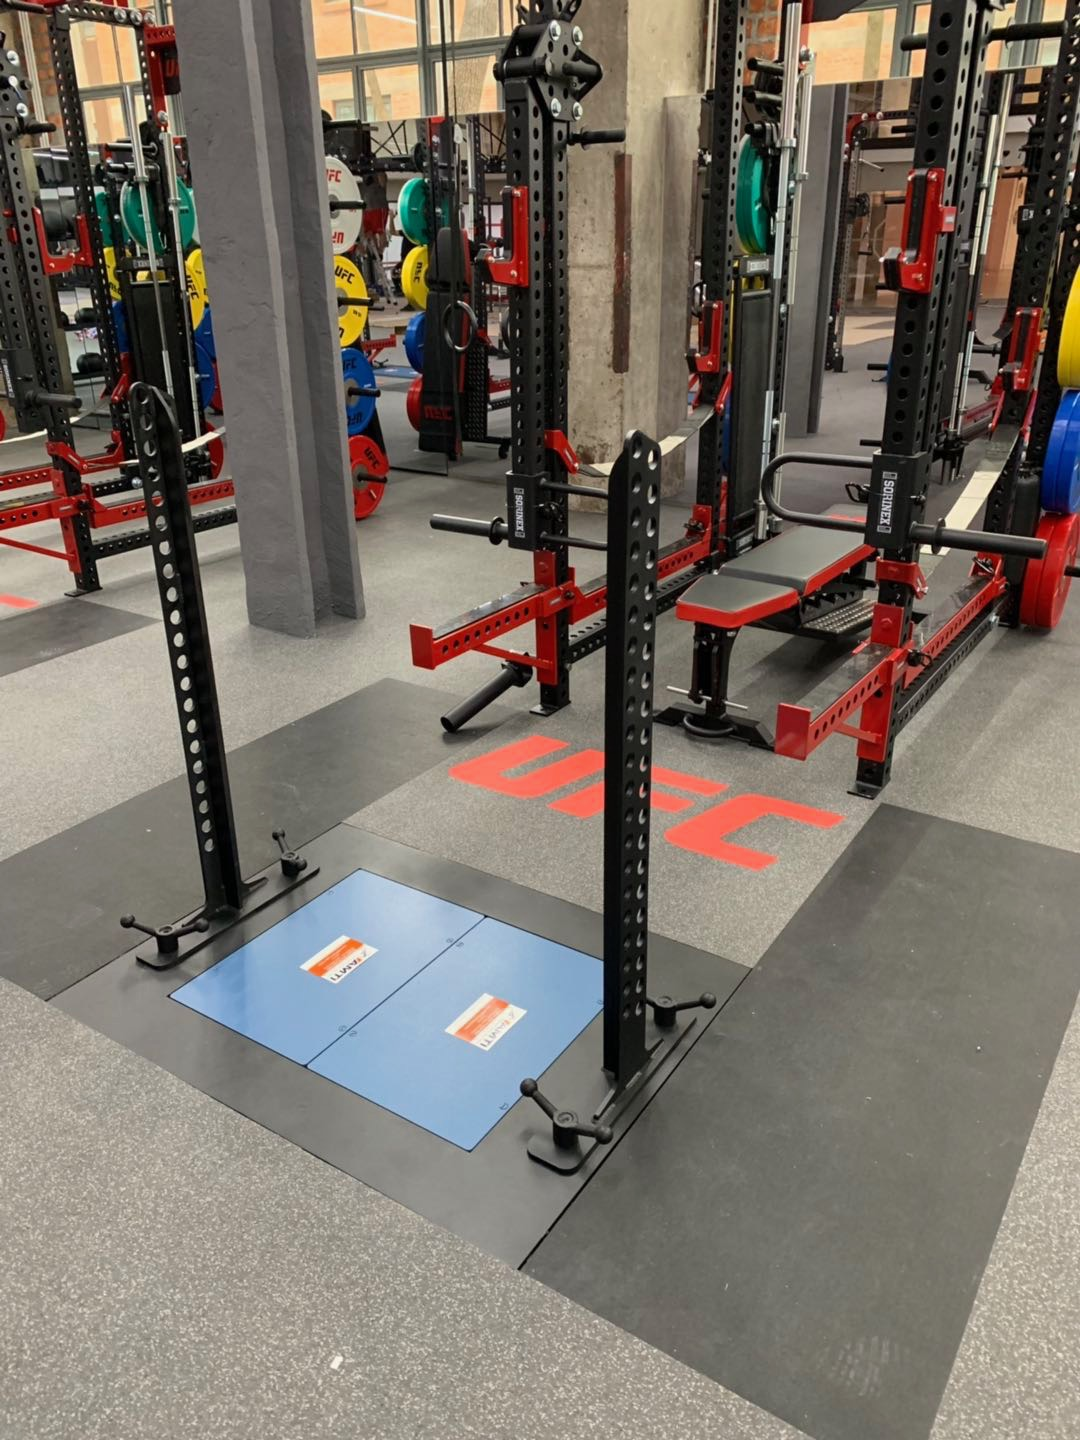
\includegraphics[height=5cm]{images/AMTI.jpeg}
    \caption{Plateforme de force (UFC)}\label{fig:AMTI}
  \end{subfigure}
  \caption{Illustration d'un logiciel et d'une plateforme de force}\label{fig:exemple_plateforme_force}
\end{figure}


\subsection{Centrales inertielles (IMU)}

Des capteurs tels que les accéléromètres, les gyroscopes et parfois les magnétomètres sont employés dans les centrales inertielles pour quantifier les mouvements corporels. 
Les accélérations linéaires sont détectées par l'accéléromètre sur les axes X, Y et Z, tandis que le gyroscope évalue les vitesses angulaires autour de ces axes. 
Lorsqu'il est intégré, le magnétomètre donne une direction absolue par rapport au champ magnétique de la Terre. 
Ces détecteurs facilitent le suivi de la position, de l'orientation et des trajets des segments du corps, y compris dans des contextes mobiles.

Les IMU sont utilisées pour l’analyse de la posture et des mouvements dans des environnements dynamiques, en dehors des laboratoires.
En sport, elles aident à optimiser les performances en analysant les mouvements des athlètes. 
En rééducation, elles permettent de suivre les progrès des patients dans leurs activités quotidiennes. 
Ces dispositifs sont également courants dans les études biomécaniques pour évaluer la stabilité dynamique et les stratégies d’équilibre.

\subsubsection{Exemples :}
\begin{itemize}
  \item \href{https://www.movella.com/products/wearables/xsens-mtw-awinda}{\textbf{Xsens MTw Awinda}}
  \item \href{https://www.noraxon.com/products/myomotion/}{\textbf{Noraxon MyoMotion}}
\end{itemize}

\begin{figure}[ht]
  \centering
  \begin{subfigure}[b]{0.45\textwidth}
    \centering
    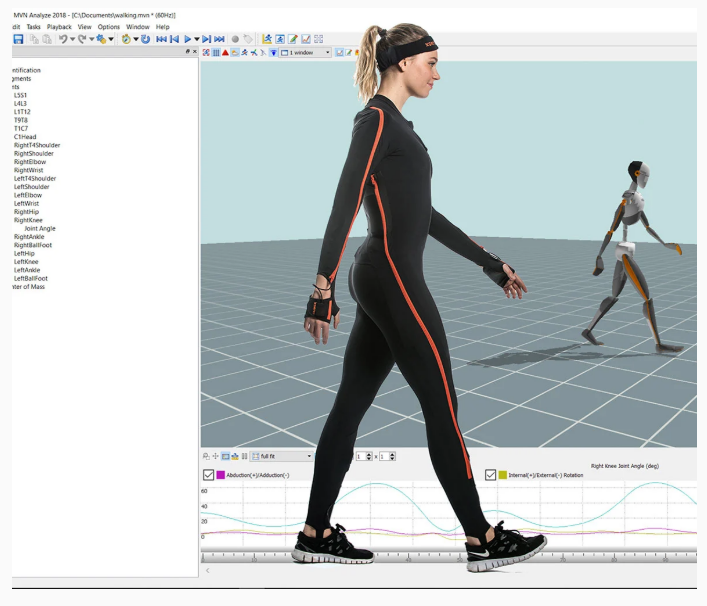
\includegraphics[height=5cm]{images/xsens.png}
    \caption{Logiciel MVN Analyse}\label{fig:mvn_analyse}
  \end{subfigure}
  \begin{subfigure}[b]{0.45\textwidth}
    \centering
    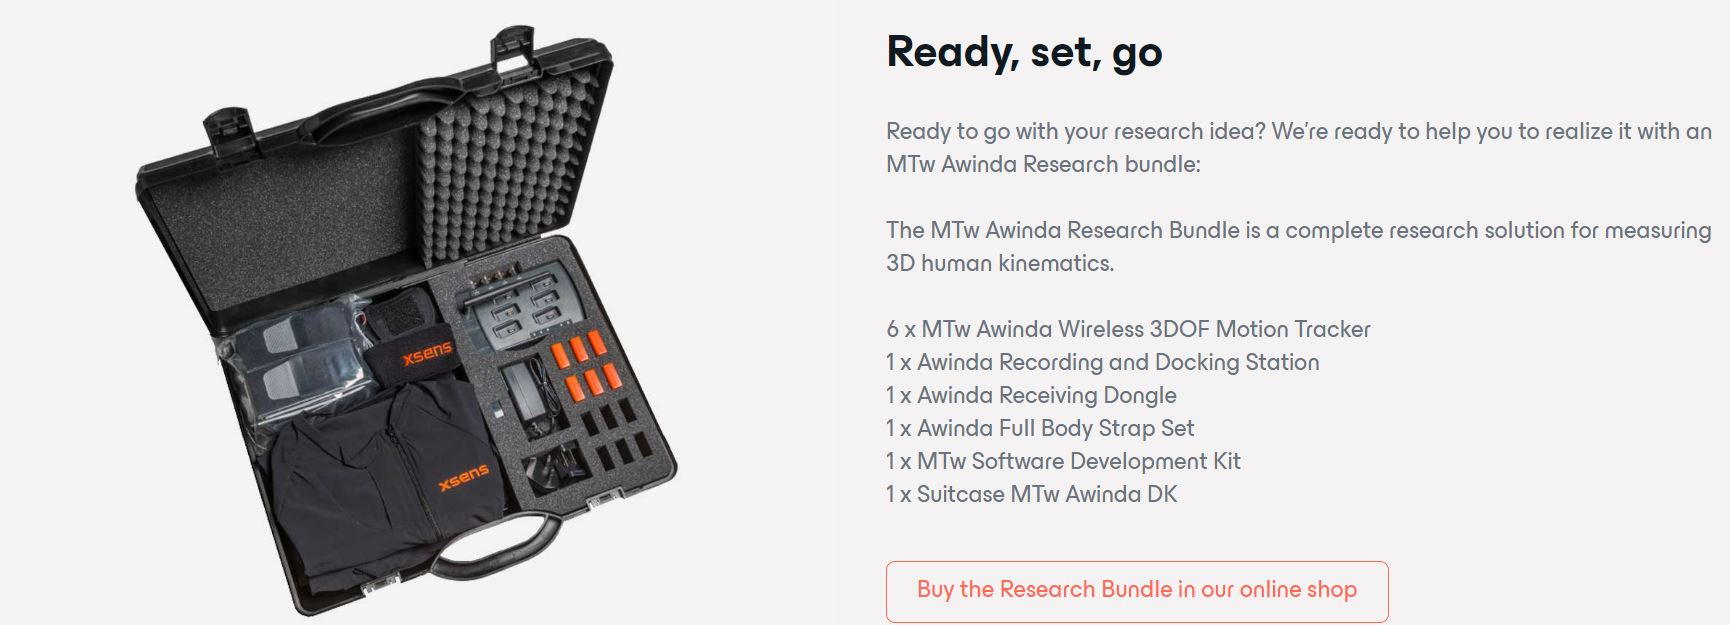
\includegraphics[height=5cm, width=\textwidth]{images/mtw_awinda.jpg}
    \caption{MTw Awinda Research bundle}\label{fig:MTw_awinda_research}
  \end{subfigure}
  \caption{Exemple de matériel utilisé dans le cadre des mesures inertielles}\label{fig:exemple_mesures_inertielles}
\end{figure}

\subsection{Plateformes stabilométriques}

Les plateformes stabilométriques, à l'instar des plateformes de force, mettent particulièrement l'accent sur l'étude des mouvements posturaux en évaluant les forces verticales et les déplacements dans les plans horizontal et vertical.
Ces plateformes disposent fréquemment d'instruments additionnels, tels que des surfaces instables ou des systèmes de visualisation interactifs, pour perturber l'équilibre et examiner les réactions compensatoires du patient.

Ces dispositifs sont utilisés pour évaluer la stabilité posturale en position debout, notamment chez des patients atteints de troubles neurologiques ou vestibulaires.
Ils sont également utilisés pour détecter les déficiences proprioceptives et pour la rééducation.
En gériatrie, ils permettent d’évaluer les risques de chute, et en sport, ils servent à optimiser les stratégies d’équilibre.

\subsubsection{Exemples : }
\begin{itemize}
  \item \href{https://www.stabilometry.com/}{\textbf{Stabilo Stabilometric Platform}}
  \item \href{https://www.natus.com/products/balancemaster}{\textbf{BalanceMaster}}
\end{itemize}


\begin{figure}[H]
  \centering
  \begin{subfigure}[b]{0.45\textwidth}
    \centering
    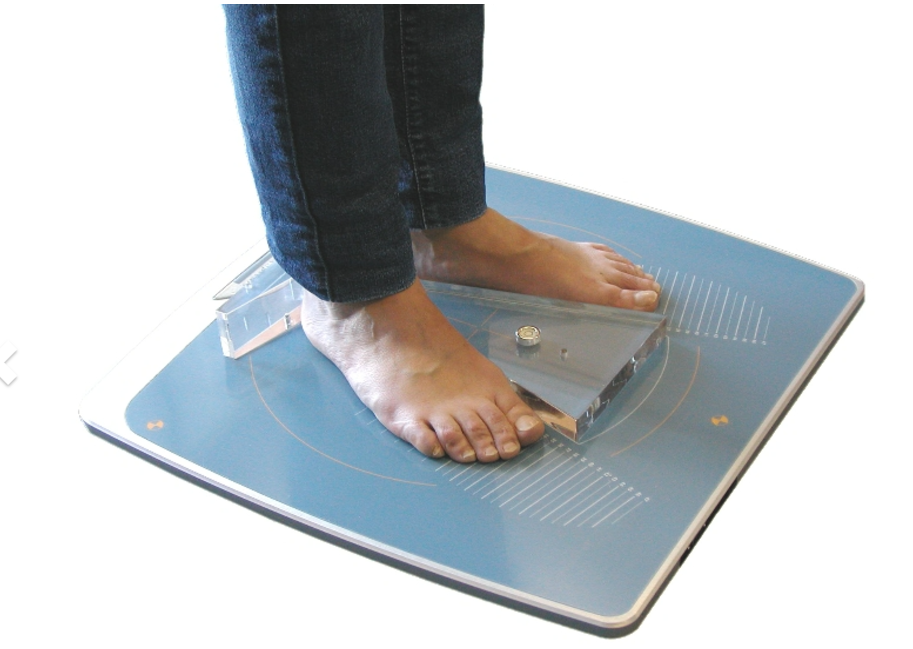
\includegraphics[height=5cm]{images/plateforme-stabilometrique.png}
    \caption{Plateforme stabilométrique}\label{fig:plateforme_stabilometrique}
  \end{subfigure}
  \begin{subfigure}[b]{0.45\textwidth}
    \centering
    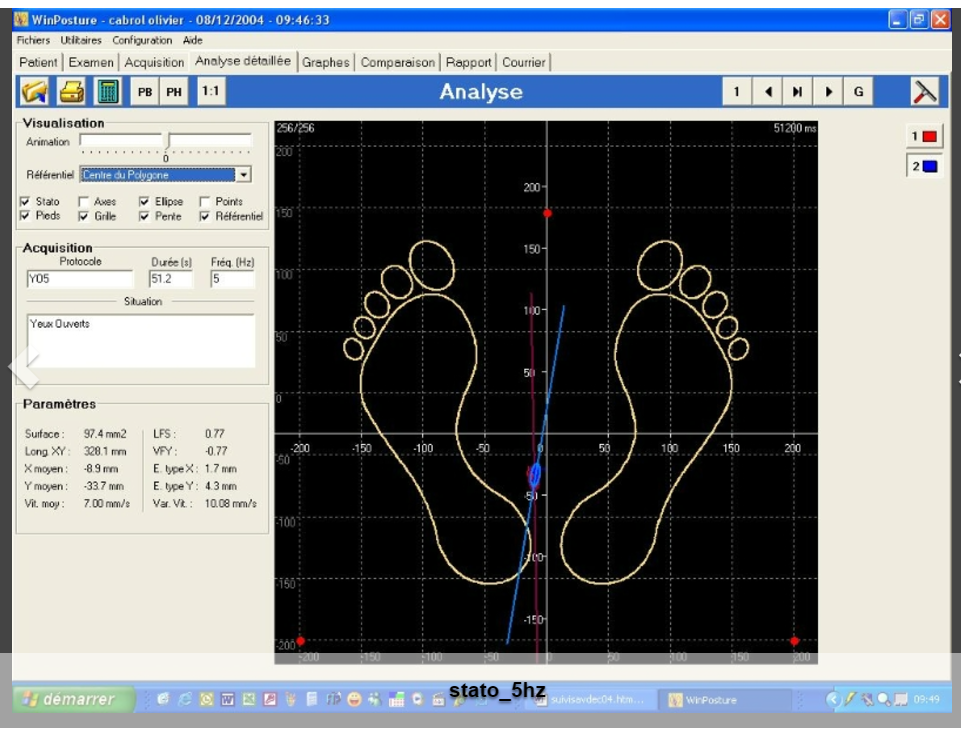
\includegraphics[height=5cm]{images/winposture}
    \caption{Logiciel Winposture}\label{fig:winposture}
  \end{subfigure}
  \begin{subfigure}[b]{0.45\textwidth}
    \centering
    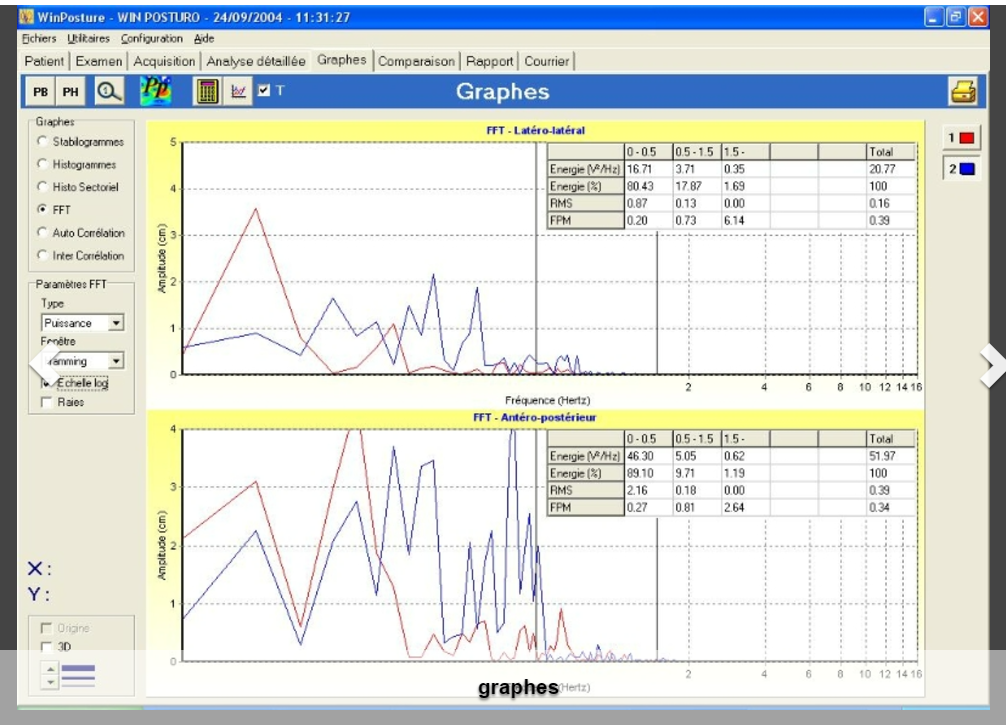
\includegraphics[height=5cm, width=\textwidth]{images/winposture-graph.png}
    \caption{Graphiques logiciel Winposture}\label{fig:winposture_graph}
  \end{subfigure}
  \caption{Exemple de dispositifs stabilométriques}\label{fig:exemple_posturographie}
\end{figure}

\subsection{Plateformes de posturographie}

Les dispositifs de posturographie évaluent les forces verticales que les pieds exercent pour déterminer les coordonnées du Centre de Pression (CdP).
Certaines plateformes intègrent des fonctionnalités dynamiques, telles que des surfaces en mouvement ou en inclinaison, afin de reproduire des perturbations de l'équilibre.

Ces plateformes servent à l'évaluation clinique de la posture, notamment dans des secteurs comme la neurologie (compréhension des troubles de l'équilibre et des affections vestibulaires), la gériatrie (pour prévenir les chutes) et la réhabilitation suite à des blessures ou interventions chirurgicales. Elles sont aussi fréquemment employées dans des recherches sur l'équilibre.

\subsubsection{Exemples :}
\begin{itemize}
  \item \textbf{BalanceTrainer Posturography System}
  \item \textbf{Stabilo}
\end{itemize}

\begin{figure}[ht]
  \centering
  \begin{subfigure}[b]{0.45\textwidth}
    \centering
    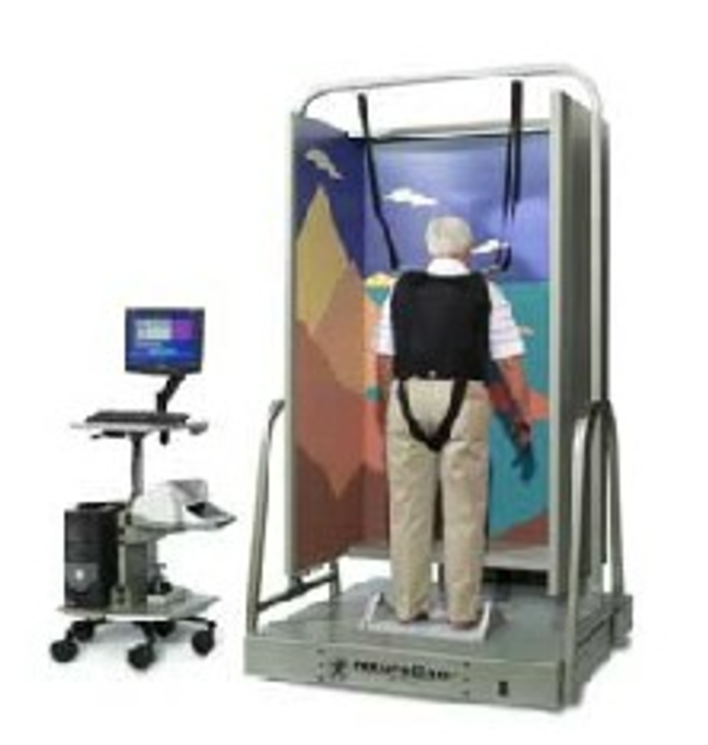
\includegraphics[height=5cm]{images/plateforme-posturographie.png}
    \caption{Plateforme posturographique}\label{fig:plateforme_posturographie}
  \end{subfigure}
  \begin{subfigure}[b]{0.45\textwidth}
    \centering
    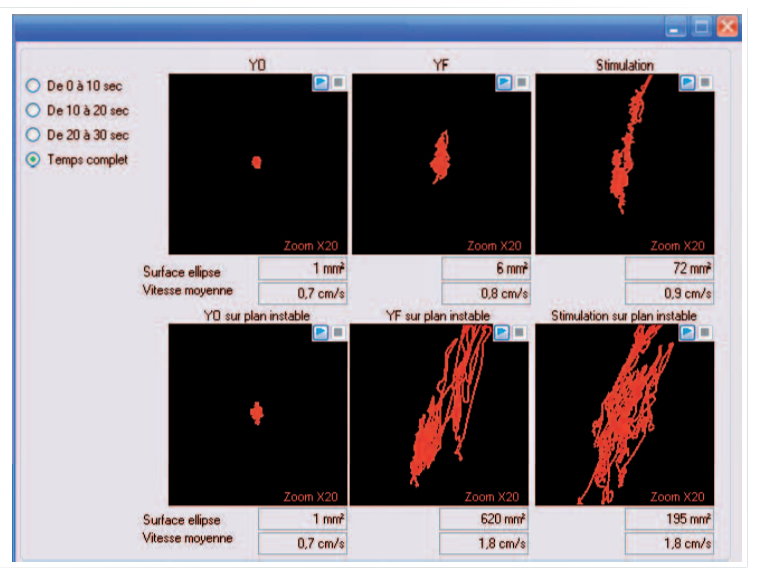
\includegraphics[height=5cm, width=\textwidth]{images/logiciel-analyse-posturographique.png}
    \caption{Logiciel d'analyse posturographique}\label{fig:logiciel_analyse_posturographique}
  \end{subfigure}
  \caption{Exemple de matériel utilisé dans le cadre d'analyse posturograpgique}\label{fig:exemple_posturographie}
\end{figure}

\subsection{Systèmes de baropodométrie}
Les dispositifs de baropodométrie évaluent les contraintes plantaires en employant des détecteurs de tension disposés sur une surface (plateformes) ou incorporés dans des semelles. 
Ces détecteurs enregistrent la distribution des forces sous les pieds et déterminent les points de tension supérieurs et inférieursD.

On utilise ces dispositifs pour examiner la dynamique et la statique du pied, principalement en podologie, orthopédie et rééducation. 
Ils servent à établir le diagnostic de maladies telles que les troubles posturaux ou les troubles du pied (comme la fasciite plantaire). 
Dans le domaine du sport, ils contribuent à perfectionner les compétences en course ou en marche.

\subsubsection{Exemples :}
\begin{itemize}
  \item \href{https://www.tekscan.com/products-solutions/systems/f-scan-system}{\textbf{Tekscan F-Scan}}
  \item \href{https://moticon.de/}{\textbf{Moticon OpenGo}}
\end{itemize}

\begin{figure}[ht]
  \centering
  \begin{subfigure}[b]{0.45\textwidth}
    \centering
    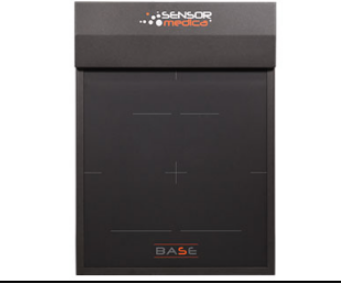
\includegraphics[height=5cm]{images/appareil-baropodometrie.png}
    \caption{Appareil de mesure de baropodométrie}\label{fig:appareil_baropodometrie}
  \end{subfigure}
  \begin{subfigure}[b]{0.45\textwidth}
    \centering
    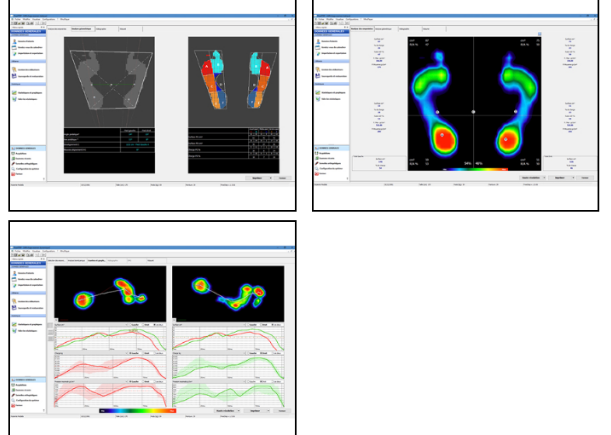
\includegraphics[height=5cm, width=\textwidth]{images/logiciel-analyse-baropodometrie.png}
    \caption{Logiciel d'analyse de baropodométrie}\label{fig:analyse_baropodometrie}
  \end{subfigure}
  \caption{Exemple de dispositifs de baropodométrie}\label{fig:exemple_baropodométrie}
\end{figure}

\subsection{Appareils d’électromyographie (EMG)}

Les dispositifs d'électromyographie consignent l'activité électrique produite par les muscles pendant leur contraction. 
Des électrodes de surface, installées sur la peau au-dessus du muscle, ou des électrodes intramusculaires, introduites directement dans le muscle, captent ces signaux. 
Les informations recueillies indiquent l'intensité, la prolongation et la fréquence de l'activation musculaire. 
Par la suite, ces signaux sont amplifiés et filtrés afin d'être examinés.

On utilise les instruments EMG pour examiner les associations musculaires et détecter les déséquilibres ou anomalies neuromusculaires. 
Ils servent à diagnostiquer des troubles comme les neuropathies ou les dystrophies musculaires en milieux hospitaliers. 
Dans le domaine sportif, l'EMG contribue à améliorer la performance musculaire et à empêcher les blessures. 
En conclusion, dans le processus de rééducation, ils surveillent les avancées des patients en évaluant la performance des exercices de renforcement.

\subsubsection{Exemples :}
\begin{itemize}
  \item \textbf{Noraxon Ultium EMG }
  \item \textbf{Delsys Trigno Wireless EMG }
  \item \textbf{BTS FREEEMG }
\end{itemize}

\begin{figure}[ht]
  \centering
  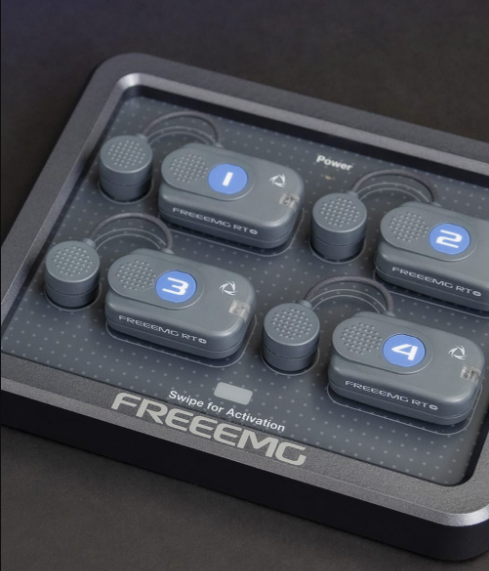
\includegraphics[height=5cm]{images/electrodes.png}
  \caption{Électrodes pour mesurer l'électromyographie}\label{fig:electrodes}
\end{figure}

\subsection{Pistes de marche électroniques}

Les pistes électroniques de marche sont des tapis munis de capteurs incorporés qui consignent les forces et la pression exercées au cours du mouvement.
Des paramètres tels que la vitesse de marche, la longueur du pas, le rythme et la symétrie font partie des informations collectées. 
Ces tapis peuvent aussi être associés à des dispositifs d'analyse vidéo ou des plateformes de force pour une analyse plus exhaustive.

Utilisées dans les laboratoires et les cliniques, ces pistes permettent d'évaluer les troubles de la marche et de suivre l'évolution des patients en réhabilitation. 
En recherche, elles offrent des données précises sur les performances locomotrices. 
Ces dispositifs sont également employés pour l'analyse des mouvements athlétiques dans le domaine du sport.

\subsubsection{Exemples :}
\begin{itemize}
  \item \href{https://www.gaitrite.com/}{\textbf{GAITRite Walkway}}
  \item \href{https://www.treadmetrix.com/}{\textbf{Treadmetrix System}}
\end{itemize}

\href{https://www.gaitrite.com/}{Voici un exemple de ce type de tapis de marche}

\subsection{Systèmes d’analyse vidéo du mouvement}

Ces dispositifs se servent de caméras (généralement infrarouges) et d'indicateurs positionnés sur les segments du corps afin d'enregistrer les mouvements dans en 2D ou 3D. 
L'analyse des trajectoires, des angles articulaires et des vitesses segmentaires est possible grâce aux informations recueillies. 
Des algorithmes d'intelligence artificielle sont également employés par certains systèmes contemporains pour réaliser des analyses sans marqueurs.

Dans le domaine de la recherche, ces dispositifs sont cruciaux pour examiner la cinématique globale du mouvement, comme c'est le cas dans les recherches biomécaniques ou les simulations sportives. 
En milieu hospitalier, ils contribuent au diagnostic des problèmes moteurs ou à la mesure de la performance fonctionnelle suite à une réhabilitation. 
Dans le domaine sportif, ils contribuent à perfectionner les méthodes des sportifs en offrant une analyse exacte de leurs mouvements.

\subsubsection{Exemples :}
\begin{itemize}
  \item \href{https://www.vicon.com/}{\textbf{Vicon Motion Systems}}
  \item \href{https://optitrack.com/}{\textbf{OptiTrack Motion Capture}}
  \item \href{https://www.qualisys.com/}{\textbf{Qualisys Motion Capture}}
\end{itemize}
Voir la vidéo : \href{https://www.youtube.com/watch?v=MTi32qJB_vo}{Laboratoire d'analyse du mouvement en 3D}

% \newpage
% \section{Plateforme similaire à notre étude}

\subsubsection{freeStep de Sensor Medica}
Cette solution logicielle complète permet l'évaluation de la distribution plantaire, l'analyse biomécanique du mouvement des membres inférieurs et l'étude de la posture corporelle. 
Elle intègre divers dispositifs pour des analyses biomécaniques et thermiques approfondies.

\begin{figure}[ht]
    \centering
    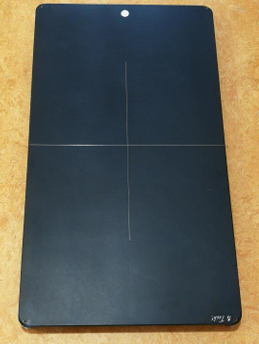
\includegraphics[width=0.5\textwidth]{images/freestep.png}
    \caption{Interface de freeStep}
    \label{fig:freestep}
\end{figure}

\end{document}
